
\chapter{Example strategies}
\label{chap:Examplestrategies}

\section{N-AFC procedures}

\element{choices}

\index{n-afc procedures}

\section{Roving} \label{sec:roving}

\index{Roving}

randomgenerator

\section{Roving another stimulus dimension}

\section{Identification by typing a sentence}

\index{Open set identification} See
\filename{examples/manual/opensetidentification.apx}. This is an
example of an open set identification task: the subject is
required to type (or repeat) the word or sentence that has been
presented(figure~\ref{fig:opensetidentification}). The results are
written to a text file.

\begin{figure}
 \centering
%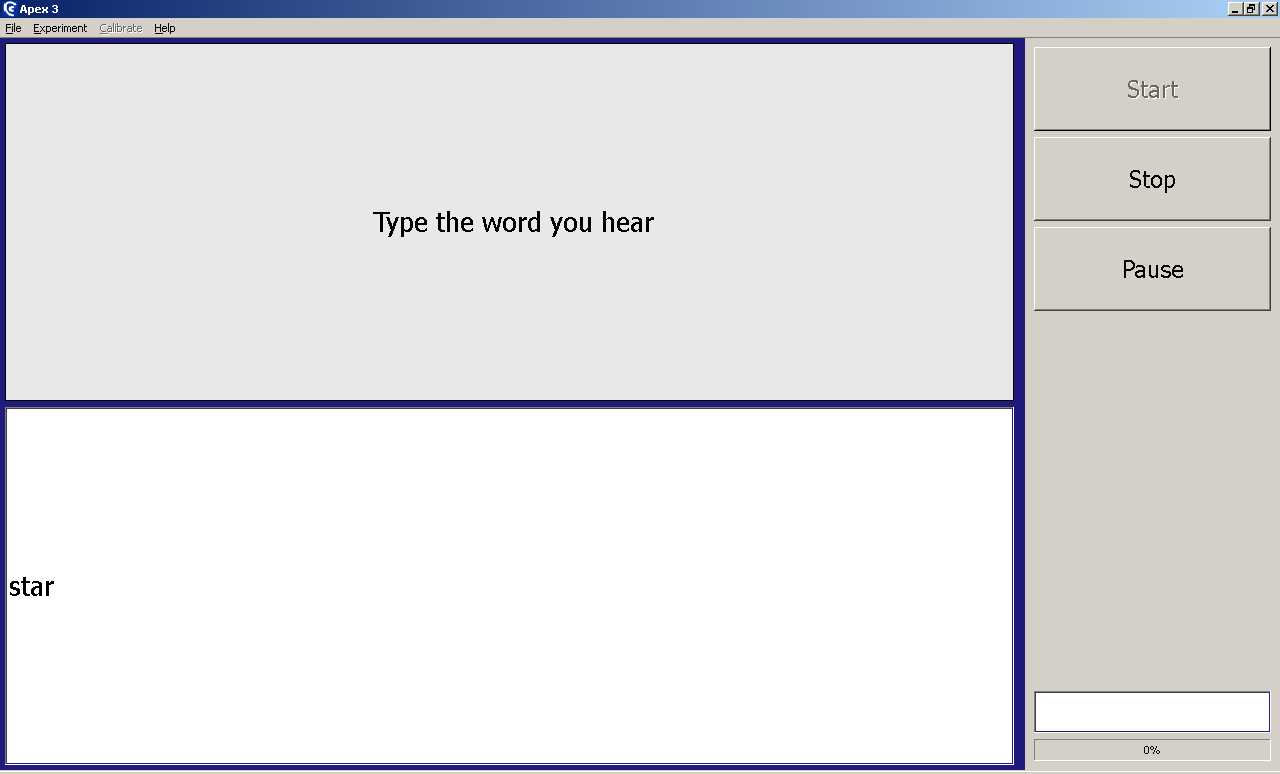
\includegraphics[width=\textwidth]{opensetidentification.png}
 \caption{Example of an open set identification experiment}
 \label{fig:opensetidentification}
\end{figure}

In order to achieve this it is necessary to adapt \element{trial},
\element{answer}, and \element{screens}.


\begin{lstlisting}
  <trial id="trial_maan">
        <answer>moon</answer>
        <screen id="screen"/>
        <stimulus id="stimulus_star"/>
      </trial>
\end{lstlisting}


\begin{lstlisting}
    <screens>
    <reinforcement>
      <progressbar>true</progressbar>
      <feedback length="600">false</feedback>
    </reinforcement>
    <screen id="screen" >
      <gridLayout height="2" width="1" id="main_layout">
        <label x="1" y="1" id="helplabel">
          <text> Type the word you hear</text>
        </label>
        <textEdit x="1" y="2" id="text" >
        </textEdit>
      </gridLayout>
      <default_answer_element>word</default_answer_element>
    </screen>
  </screens>
\end{lstlisting}


\section{Practice}

\index{Practice}

See \filename{examples/manual/trainprocedure.apx}. Here the
subject clicks on an interval and a stimulus is presented. This
can be done as often as he/she wishes.

To achieve this \element{procedure
xsi:type="apex:trainingProcedureType"} should be used.

\section{Higlighting} example threshold
procedure, 2 interval, 1 tone

alle soorten van highlighting (theoretisch deel)

\subsection{Interleaving procedures}

multiprocedure



cmd line parameter


\begin{itemize}
 \item procedure
\item corrector \item ...
\end{itemize}
